%\documentclass[3p,twocolumn]{elsarticle}
\documentclass[review]{elsarticle}
\usepackage{graphicx}
\usepackage[export]{adjustbox}%for left right graphic adjust
\usepackage{amsmath}
\usepackage{float}
\usepackage{overpic}
\usepackage{contour}
\usepackage{color}
\graphicspath{ {images/} }

\usepackage[T1]{fontenc}
%\usepackage[utf8]{inputenc}
\usepackage{lineno,hyperref}
\modulolinenumbers[5]

\journal{Journal of \LaTeX\ Templates}

%%%%%%%%%%%%%%%%%%%%%%%
%% Elsevier bibliography styles
%%%%%%%%%%%%%%%%%%%%%%%
%% To change the style, put a % in front of the second line of the current style and
%% remove the % from the second line of the style you would like to use.
%%%%%%%%%%%%%%%%%%%%%%%

%% Numbered
%\bibliographystyle{model1-num-names}

%% Numbered without titles
%\bibliographystyle{model1a-num-names}

%% Harvard
%\bibliographystyle{model2-names.bst}\biboptions{authoryear}

%% Vancouver numbered
%\usepackage{numcompress}\bibliographystyle{model3-num-names}

%% Vancouver name/year
%\usepackage{numcompress}\bibliographystyle{model4-names}\biboptions{authoryear}

%% APA style
%\bibliographystyle{model5-names}\biboptions{authoryear}

%% AMA style
%\usepackage{numcompress}\bibliographystyle{model6-num-names}

%% `Elsevier LaTeX' style
\bibliographystyle{elsarticle-num}
%%%%%%%%%%%%%%%%%%%%%%%

\begin{document}

\begin{frontmatter}

\title{Extending the Dynamic Range of Electronics in a Time Projection Chamber}

%% Group authors per affiliation:
%\author{Elsevier\fnref{myfootnote}}
%\address{Radarweg 29, Amsterdam}
%\fntext[myfootnote]{Since 1880.}

%% or include affiliations in footnotes:
\author[msu,nscl]{J. Estee}
\author[msu,nscl]{W.G. Lynch}
\author[china1,china2]{R. Wang}
\author[msu,nscl]{J. Barney}
\author[msu,nscl]{G. Cerizza}
\author[kor]{B. Hong}
\author[riken]{T. Isobe}
\author[nscl]{G. Jhang}
\author[kyoto]{M. Kaneko}
\author[riken]{M. Kurata-Nishimura}
\author[krakow]{P. Lasko}
\author[kor]{J. W. Lee}
\author[krakow]{J. \L ukasik}
\author[a&m]{A.B. McIntosh}
\author[kyoto]{T. Murakami}
\author[krakow]{P. Paw\l owski}
\author[poland]{K. Pelczar}
\author[nscl]{C. Santamaria}
\author[riken]{D. Suzuki}
\author[nscl]{M. B. Tsang}
\author[a&m]{S.J. Yennello}
\author[tsing]{Y. Zhang}
\author[]{and the S$\pi$RIT collaboration}

\address[msu]{Dept. Physics and Astronomy, Michigan State University, East Lansing, Michigan, 48824, USA }
\address[nscl]{National Superconducting Cyclotron Laboratory, East Lansing, Michigan, 48824, USA}
\address[kor]{Department of Physics, Korea University, Seoul 136-703, Republic of Korea }
\address[riken]{RIKEN Nishina Center, Hirosawa 2-1, Wako, Saitama 351‐0198, Japan }
\address[kyoto]{Department of Physics, Kyoto University, Kita-shirakawa, Kyoto 606-8502, Japan }
\address[krakow]{Institute of Nuclear Physics PAN, ul. Radzikowskiego 15231-342 Krak\'{o}w, Poland}
\address[a&m]{Dept. of Physics and Astronomy, Texas A$\&$M University, College Station, TX 77843, USA }
\address[tsing]{Department of Physics, Tsinghua University, Beijing 100084, P. R. China}
\address[poland]{Faculty of Physics, Astronomy and Applied Computer Science, Jagiellonian University, ul. Go\l \k{e}bia 24, 31-007 Krak\'{o}w}
\address[china1]{State Key Laboratory of Radiation Medicine and Protection, School of Radiation Medicine and Protection, Soochow University, Suzhou 215123, China}
\address[china2]{Collaborative Innovation Center of Radiological Medicine of Jiangsu Higher Education Institutions, Suzhou 215123, China}



\begin{abstract}

As Time Projection Chambers (TPCs) become widely used in low to intermediate heavy ion collisions, of around 300 MeVA, the mass and momentum range covered by the resulting particles cover a wide dynamic range. Many TPCs currently only have a single gain output with a fixed dynamic range. In a recent set of experiments using the SAMURAI Pion-Reconstruction and Ion-Tracker (S$\pi$RIT) TPC, it was important to simultaneously measure relativistic pions and heavy ion tracks from the same collisions. As a tracks energy loss is collected and multiplied by the anode wires, the charge is spread out onto a distribution on the TPC read out pads. If the avalanche on a wire is high enough, the charge collected on a pad will saturate the electronics, though only for pads directly underneath the avalanche; pads further away in the distribution will not be saturated. Using these unsaturated pads and the known distribution function, we recover the saturated pads, increasing the dynamic range by a factor of 10.

\end{abstract}

\begin{keyword}
\texttt{elsarticle.cls}\sep \LaTeX\sep Elsevier \sep template
\MSC[2010] 00-01\sep  99-00
\end{keyword}

\end{frontmatter}

\linenumbers

\section{Introduction} 
 The particles resulting from low to intermediate energy heavy ion collisions cover a large range in energy losses from very small energy losses, for minimum ionizing particles, to much higher energy losses, for slower moving, heavy fragments. Figure \ref{fig:intro} shows the range of momenta typically observed in intermediate energy collisions, around 300 MeVA, and the energy loss range involved.  
 
  Measuring the full range in energy losses have motivated the development of large dynamic range electronics, which are able to switch between high and low gains covering a very large dynamic range; however, many current Time Projection Chambers (TPCs) readout electronics have a single gain output, presenting a problem for the readout of such devices.
 
 Several techniques have been employed to increase the dynamic range for energy losses in TPCs. In the EOS TPC \cite{eos}, a larger dynamic range was achieved by lowering the voltage on selected anode wires, decreasing the gas amplification on those wires. In the prototype Active Target TPC (PAT-TPC) an equivalent reduction in gain was achieved by lowering the electronics gain for some of the readout channels. 
me sections, and optimizing the gain for strongly ionizing particles in others. For strongly ionizing particles, lowering the gain improves the momentum resolution, while worsening the dE/dx resolution, and vice versa for weakly ionizing particles. 
 
 These strategies have drawbacks because in many applications the experiment's requirements cannot accept the associated degradation in the dE/dx
resolution, or the momentum resolution. Finding the solution to this problem has motivated the development of software based analysis that will extend the dynamical range of TPCs; we illustrate an alternate approach to expand the dynamic range within the context of a standard multi-wire TPC, without the need of extra hardware or dedicating regions of lower gain. 
 
 Many TPC readout electronics have a single gain output with a dynamic range (defined the ratio of the maximum signal to the electronic noise) of no more than 1000:1. In our case the maximum signal to noise was about 700:1. We required the smallest signal of minimum ionizing particles (m.i.p.) to be 20:1, setting the dynamic range to be 35 times m.i.p. Figure \ref{fig:intro} illustrates the effect saturation has on the measured momentum of the particles. The shaded region shows where 35 times that of the minimum ionizing pion signal where we could expect saturation to occur. While the pion's momentum range can fully be measured, without saturation effects, heavier particles would be harder to resolve in dE/dx at lower momentum.

 
 
\begin{figure}[H]
\includegraphics[width=\linewidth]{intrographic}
\caption{}
\label{fig:intro}
\end{figure}

\paragraph{1.1 TPC Overview}
We begin our discussion by describing some basic properties of the SAMURAI Pion Reconstruction and Ion-Tracker (S$\pi$RIT) TPC \citep{shane}. For the following discussion we have defined the +x axis to point to the left of the beam, the -y axis to point down into the drift volume, and the +z axis to point along the beam. 

\begin{figure}[H]
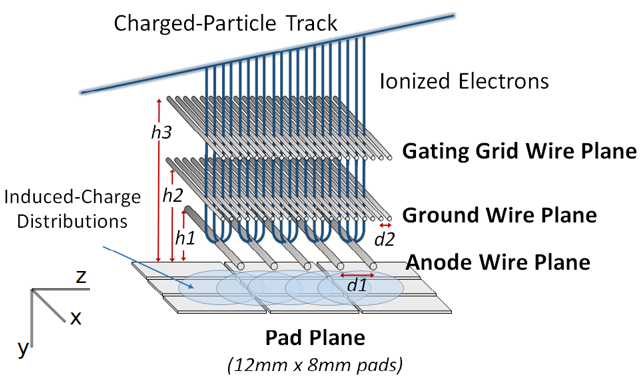
\includegraphics[width=\linewidth]{padwire}
\caption{Cartoon graphic showing the 3 wire planes and a section of the pad plane. h3 =14 mm, h2 = 8 mm, h1 = 4 mm, d2 = 1 mm, d1 = 4 mm. This graphic is inverted from the actual wire planes and pad plane to display the perspective easier.}
\label{fig:padwire}
\end{figure}

\paragraph{Pad plane} 
The S$\pi$RIT TPC pad plane consists of a 2-dimensional plane of rectangular charge sensitive pads with an x dimension of of 8 mm wide, and a z dimension of 12 mm. These pads are laid out on a grid measuring 112 by 108 pads with a total area of 1344 mm x 864 mm.

\paragraph{Wire planes}
Illustrated in Figure \ref{fig:padwire}, the S$\pi$RIT TPC consists of three wire planes below the pad plane, with wires aligned along the x-axis. The first wire plane operates as an ion-gate or gating grid; the second wire plane is held at ground, with both wire planes serving to isolate the drift volume from the gas amplification stage. 

Closest to the pad plane is the high voltage, anode wire plane, consisting of 20 $\mu$m diameter wires spaced 4 mm apart, and set at a height of 4 mm from the pad plane. Near the vicinity of these wires an avalanche occurs multiplying the secondary electrons drifting up from the drift volume, created from the track's energy loss in the detector gas. When these secondary electrons reach the anode wires, they are multiplied on the order of 1000 times creating electron and ion pairs. It is the motion of these slow moving ions, drifting away from the anode wires, that induce images charges on the read out pads above. The distribution of image charges on the pad plane is fixed by the geometry of the anode wire grid, and its distance from the pad plane. 

The anode wires are sectioned off into 14 independent sections, each containing 26 wires; 12 sections were biased to 1460 V. This setting was optimized to ensure m.i.p. particles such as pions would at have a signal to noise ratio of around 20:1. The two remaining sections were biased to 1214 V due to high current issues, reducing the gas gain by a factor of 10 times as compared to the other anode sections. Lowering the anode wires effectively extended the dynamic range, though unnecessary for the following method to be discussed, and allowed for a direct validation of the method's success. 

\paragraph{Generic Electronics for TPCs}
Signals in the S$\pi$RIT TPC are amplified and digitized by the recently developed Generic Electronics for TPCs (GET) \cite{get}.  Short cables transmit the signals from the pads to the inputs of the AGET chips. Each AGET chip services 64 pads (63 pads are connected in our case), contains a pre-amplifier, and a Switched Capacitor Array (SCA), with a maximum of 512 time buckets sampling at 1 to 100 MHz. Four AGET chips are mounted on one AsAd (ASIC and ADC) motherboard. The gain of each AGET can be configured as 0.12, 0.24, 1.0, or 10 pC over the whole dynamic range, and the ADCs on each AsAd board provides 12 bit resolution. The peaking times of the shaping amplifiers can be set to 69, 117, 232, 501, 720, or 1014 ns. In this experiment, the gain was set to the highest setting, 0.12 pC, the peaking time 117 ns, and the width of the time bucket was 40 ns. The Aget 2.0, asad 2.1, and cobo 1.0 firmware versions were used. The variations in the electronics were calibrated by measuring the response of each channel to a injected reference pulse, covering the full dynamic range of each channel. 

\begin{figure}[H]
\includegraphics[width=\linewidth]{defofavalanche}
\caption{Cartoon graphic of avalanche event on an anode wire over one layer of pads. The estimate of the position of the avalanche is given by $\bar{x}$  the mean. The position from the center to each pad to the $\bar{x}$ position is given as $\lambda_i$.}
\label{fig:av}
\end{figure}

\begin{equation}\label{eq:1}
\begin{split}
PRF(\lambda_i) 
& = \frac{q_i(\lambda_i)}{Q} \\
& Q=\sum_i q_i \\
& \bar{x}= \frac{\sum_i x_i q_i}{Q}\\
& \lambda_i=x_i-\bar{x} \\
\end{split}
\end{equation}

\begin{equation}\label{eq:gatti}
\begin{split}
PRF_{gatti}(\lambda)
& = \frac{K_{1}}{K_{2}\sqrt{K_{3}}}\bigl[arctan(\sqrt{K_{3}}tanh\bigl[K_{2}\bigl(\frac{\lambda}{h}+\frac{w}{2h}\bigr)\bigr]) \\
& - arctan(\sqrt{K_{3}}tanh\bigl[K_{2}\bigl(\frac{\lambda}{h}-\frac{w}{2h}\bigr)\bigr])\bigr] \\
& K_3 = .48\\
& K_2 = \frac{\pi}{2}\left(1-\frac{\sqrt{K_{3}}}{2}\right)\\
& K_1 = \frac{K_{2}\sqrt{K_3}}{4 atan(\sqrt{K_3})}\\
\end{split}
\end{equation}

\begin{equation}\label{eq:gaus}
PRF_{gaus}(\lambda) = .5\left[erf\left(\frac{\lambda+\frac{w}{2}}{\sqrt{2}\sigma}\right) - erf\left(\frac{\lambda-\frac{w}{2}}{\sqrt{2}\sigma}\right) \right]
\end{equation}


\section{Pad Response Function}
\paragraph{Experimental PRF}



The distribution resulting from an electron avalanche is 2-dimensional; the charge collected on each pad being the integral of that distribution over the pad's dimensions. It is impractical to calculate the avalanche position using the full 2-dimensional distribution; instead we calculate the center of gravity of charge along the direction most perpendicular to the track, giving the best momentum resolution. For a track traversing in the z direction we would cluster along the x, and vice versa.

 A semi-empirical equation, for both x and z directions of a simple multi-wire TPC, is given by Gatti \cite{gatti}, and also summarized in \cite{blumrol}. The integral of the charge distribution, over one pad, is referred to as the Pad Response Function (PRF); given for the Gatti distribution by equation \ref{eq:gatti} in \cite{blumrol}. The overlap of of the PRFs of adjacent wires and diffusion of the primary electrons correlate the charge observed causing deviations from the expected Gatti PRF, also analytic PRFs only exist for classical multi-wire TPCs; in these cases an effective PRF may be calculated from experimental data. An effective PRF is calculated and used here in the following. 

We postulate that the PRF is only a function of the total charge deposited on the wire Q and the displacement $\lambda$; the difference in position of the center of the $i^{th}$ pad, $x_i$, to the mean position $\bar{x}$, given by equation \ref{eq:1} and illustrated in Figure \ref{fig:av}. Averaging over many events, the resulting experimental PRF for the S$\pi$RIT TPC is shown in figure \ref{fig:expprf}. A Gaussian function, equation \ref{eq:gaus}, was used to fit to the experimental PRF; the agreement with the data is better than with the Gatti distribution. 

\begin{figure}[H]
\begin{overpic}[width=\linewidth]{expprf}
\put(61,55){\contour{white}{ PRF${}_{gaus}(\lambda)$ eq. \ref{eq:gaus}  }}
\put(61,49){\contour{white}{ PRF${}_{gatti}(\lambda)$ eq. \ref{eq:gatti} }}
\end{overpic}
\caption{Experimental pad response function. Constructed from total number of pads $>$=3. }
\label{fig:expprf}
\end{figure}


%\begin{figure}[H]
%\includegraphics[width=\linewidth]{expprf}
%\caption{Experimental pad response function. Constructed from total number of pads $>$=3. }
%\label{fig:expprf}
%\end{figure}


\paragraph{Method of Desaturation}
Figure \ref{fig:satpad} shows a typical situation of saturated signals. When an avalanche causes a large induced signal, the pad directly underneath collects the largest charge becoming saturated, pads further away experience smaller, non saturating charges; $q_{2'}$, $q_{3'}$ and  $q_{1}$, $q_{4}$ respectively as indicated in figure \ref{fig:satpad}. 

We will use the term ``desaturation" for our process of correcting the charge values of the saturated pads.

The charge deposited on each pad, though saturated, must satisfy the PRF distribution. The small non-saturated tails, $q_{1}$ and $q_{4}$, we perform a $\chi^2$ fit to find the unknown charges of the saturated pads. 

%The data points of the $\chi^2$ fit are the unsaturated pads,  $q_{1}$ and $q_{4}$, and the unknown parameters of the fit are $q_{2'}$ and $q_{3'}$ with the expected values coming from the PRF described above. The values of $q_{2'}$ and $q_{3'}$ at the minimum of the $\chi^2$ would be the best estimate for the saturated pads. 

\begin{figure}[H]
\includegraphics[width=\linewidth]{saturated_pads}
\caption{•}
\label{fig:satpad}
\end{figure}

\section{Experimental data}
Two sets of data were used for the testing and validation of this method. A cocktail beam consisting of (p,d,t,${}^3He$,${}^4He$,${}^6Li$,${}^7Li$) light charged particles was injected into the TPC for calibration purposes, and tuned to two different ridgidity, $\beta\rho$, settings. The momentum resolution was approximately 1\%, as determined by the slits of the BigRIPS fragment separator of the Radioactive Isotope Beam Factory (RIBF) in RIKEN. A thick 21 mm thick aluminum target was inserted for part of the lower $\beta\rho$ setting, further reducing the energy of the beam for a third calibration point. 

In a typical cocktail event, one particle enters the TPC volume at a time and parallel to the pad plane; an ideal case for momentum and dE/dx determination as it does not suffer from inefficiencies of high multiplicity events seen in the collision experimental data.  

\begin{figure}[H]
\includegraphics[width=\linewidth]{data.pdf}
\caption{Pad plane projection for a collision event in the TPC. Highlighted by red arrows are two regions of anode wires which had a reduced voltage of 1214 V. The voltage of the rest of the TPC anode wires are 1460 V. The reduction in voltage reduces the gain by a factor of about 10x. }
\label{fig:data}
\end{figure}

The other type of data was the collision of a ${}^{132}$Sn beam onto a ${}^{124}$Sn target triggered on central nuclear collisions. Shown in figure \ref{fig:data} is the typical pad plane response for a central nuclear collision. During the experiment the voltages of two anode sections (as indicated by red arrows in figure \ref{fig:data}) were biased to 1214 V. The gain of these sections were also reduced by a factor of about 10 times, as compared with the other sections which were biased to 1460 V. We refer to the 1460 V region as high gain and the 1214 V region as low gain. 


\section{Results}
\paragraph{Low gain vs corrected high gain}

Tracks which saturate pads in the high gain region are not saturated in the low gain region; by comparing the dE/dx values of these two sections, we can directly measure the success of the high gain region's desaturation using the method described above.  

\begin{figure}[H]
\includegraphics[width=\linewidth]{dedxcompare_nodesat}
\caption{The uncorrected high gain dE/dx vs low gain dE/dx collision data.  }
\label{fig:lowvshigh_raw}
\end{figure}
 
In figure \ref{fig:lowvshigh_raw}, the effect of saturation can be seen in the high gain region for the uncorrected data. For signals below 400 ADC/mm the electronics are not saturated, and therefore the high and low gain sections agree. The data starts to saturate above 400 ADC/mm in the high gain channels eventually reaching a plateau; the low gain sections have not saturated and provide true dE/dx values.
 After applying the desaturation method, the correlation between the high and low gain sections is restored, as seen in figure \ref{fig:lowvshigh_desat}. We believe the correction to at least about 2000 ADC/mm, increasing the dynamic range by a factor of 5 times.

\begin{figure}[H]
\includegraphics[width=\linewidth]{dedxcompare_new}
\caption{The corrected high gain dE/dx vs low gain dE/dx for collision data.  }
\label{fig:lowvshigh_desat}
\end{figure}

\paragraph{Particle Identification (PID)}


\begin{figure}[H]
\begin{overpic}[width=\linewidth]{cocktail_sat.png}
\put(22,15){\contour{white}{\Large p} }
\put(27,20){\contour{white}{\Large d} }the
\put(31,25){\contour{white}{\Large t} }
\put(30,31){\contour{white}{\large ${}^{3}$He} }
\put(33,35){\contour{white}{\large ${}^{4}$He} }
\put(60,27){\contour{white}{\large ${}^{6}$Li} }
\end{overpic}
\caption{Uncorrected cocktail data.}
\label{fig:cocktail_raw}
\end{figure}

%\begin{figure}[H]
%\includegraphics[width=\linewidth]{cocktail_sat.png}
%\caption{Uncorrected cocktail data.}
%\label{fig:cocktail_raw}
%\end{figure}

\begin{equation}
\label{eq:calib}
\frac{ADC}{mm} = 20. \frac{keV}{cm}
\end{equation}

Comparing the low to high gain sections provides a direct measurement for determining the success of the desaturation technique, but the goal would be to improve the particle identification (PID). In the following PID plots the red lines represent the most probable energy loss as given by Geant4 straggling functions after calibration to the experimental data, resulting from a linear fit to the uncorrected data, given in equation \ref{eq:calib}.

There are pronounced PID lines of several particle species in both the uncorrected and corrected cocktail beam PID in figures \ref{fig:cocktail_raw} and \ref{fig:cocktail_desat}. Three ovals around 1700 and two near 900 [MeV/c/Z] correspond to the three B$\rho$ settings injected into the TPC. The tails of the PID lines resulting from the particle losing its initial energy, passing through the walls and other materials outside the main detector volume; therefore lowering their initial momentum. 

The uncorrected data in figure \ref{fig:cocktail_raw} shows the effects of saturation; the PID lines deviate from their theoretical expectations starting around 400 ADC/mm eventually reaching a plateau. After applying the desaturation technique, we see a large improvement; most notably the He and Li particles, which suffer the most from saturation. A more subtle improvement of the lighter particles, (p,d,t), can also be seen in the PID lines at lower momentum.

\begin{figure}[H]	
\begin{overpic}[width=\linewidth]{cocktail_desat.png}
\put(22,15){\contour{white}{\Large p} }
\put(27,20){\contour{white}{\Large d} }
\put(31,25){\contour{white}{\Large t} }
\put(30,31){\contour{white}{\large ${}^{3}$He} }
\put(34,35){\contour{white}{\large ${}^{4}$He} }
\put(60,27){\contour{white}{\large ${}^{6}$Li} }
\end{overpic}
\caption{Corrected (desaturated) cocktail data.}
\label{fig:cocktail_desat}
\end{figure}

%\begin{figure}[H]
%\includegraphics[width=\linewidth]{cocktail_desat.png}
%\caption{Corrected (desaturated) cocktail data.}
%\label{fig:cocktail_desat}
%\end{figure}


 
Looking at the collision data, in figures $\ref{fig:data_raw}$ and $\ref{fig:data_desat}$, we also see a similar result. Of course the collision data PID suffers from background and inefficiencies than the cocktail beam; nevertheless we can see a similar improvement in the PID lines when comparing the uncorrected to after the desaturation has been applied. Since the separation of particle species at lower momenta and the separation of the Li species into ${}^{6}$Li and ${}^{7}$Li, whereas there was little to no separation before. 

\begin{figure}[H]	
\begin{overpic}[width=\linewidth]{data_sat.png}
\put(22,15){\contour{white}{\Large p} }
\put(27,20){\contour{white}{\Large d} }
\put(31,25){\contour{white}{\Large t} }
\put(30,31){\contour{white}{\large ${}^{3}$He} }
\put(34,35){\contour{white}{\large ${}^{4}$He} }
\put(60,27){\contour{white}{\large ${}^{6}$Li} }
\end{overpic}
\caption{Uncorrected collision data.}
\label{fig:data_raw}
\end{figure}

%\begin{figure}[H]
%\includegraphics[width=\linewidth]{data_sat.png}
%\caption{Uncorrected collision data.}
%\label{fig:data_raw}
%\end{figure}


\begin{figure}[H]	
\begin{overpic}[width=\linewidth]{data_desat.png}
\put(22,15){\contour{white}{\Large p} }
\put(27,20){\contour{white}{\Large d} }
\put(31,25){\contour{white}{\Large t} }
\put(30,31){\contour{white}{\large ${}^{3}$He} }
\put(34,35){\contour{white}{\large ${}^{4}$He} }
\put(60,27){\contour{white}{\large ${}^{6}$Li} }
\end{overpic}
\caption{Corrected (desaturated) collision data.}
\label{fig:data_desat}
\end{figure}

%\begin{figure}[H]
%\includegraphics[width=\linewidth]{data_desat.png}
%\caption{Corrected (desaturated) collision data.}
%\label{fig:data_desat}
%\end{figure}


\section{Conclusion}

Saturation reduces dE/dx resolution and even the maximum charge observable inside of a TPC we have shown that some of the saturation is recoverable. Since the Pad Response Function of the TPC is fixed by the anode wire geometries, an experimental PRF can be calculated from the unsaturated experimental data. The pads resulting from an avalanche on a wire must follow this PRF even if the electronics of some channels directly under the avalanche are saturated, pads further away are not saturated; using these unsaturated pads we perform applying a $\chi^2$  fit the unknown saturated pads to this PRF function. 

Looking at the PID lines, and also making a direct comparison to some low gain sections of the TPC, we were able to extend the dynamic range of our electronics by a factor of about 5 times. This improved PID will allow for us to extend the momentum distributions of all species to lower momenta than what was previously available. 

\section{Acknowledgments}
This work was supported by the U.S. Department of Energy under Grant Nos.  DE-SC0004835,  DE-SC0014530, DE-NA0002923,  US  National Science Foundation Grant  No.  PHY-1565546, the  Japanese  MEXT  KAKENHI(Grant-in-Aid  for  Scientific  Research  on  Innovative  Areas)  grant  No. 24105004, and Polish National Science Center (NCN), under contract Nos. UMO-2013/09/B/ST2/04064 and UMO-2013/10/M/ST2/00624. The computing resources for analyzing the data was provided by the HOKUSAI-GreatWave system at RIKEN. 

\section*{References}

\bibliography{mybibfile}

\end{document}